\documentclass{subfiles}
\begin{document}
\begin{wrapfigure}[14]{r}[0pt]{0.4\textwidth}
    \centering
    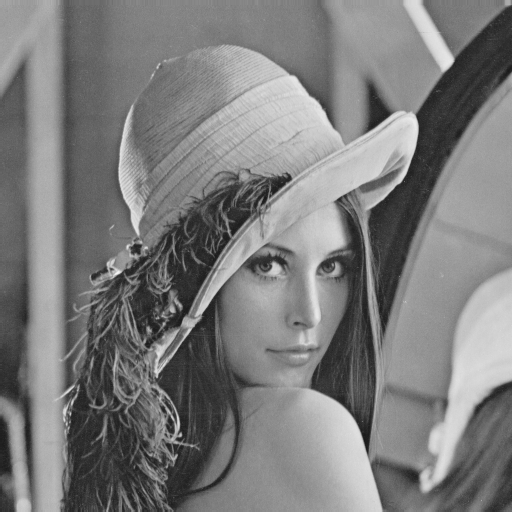
\includegraphics[width = 0.35\textwidth]{../../Figure/Other/Lena/Lena.png}
    \caption{Immagine base: Lena.}
    \label{fig:3.1}
\end{wrapfigure}
Lavorando con le immagini potrebbe essere necessario dover modificare le stesse in qualche modo: accentuando i dettagli o evidenziandone i contorni; ma come fare ciò?
La risposta: tramite l'applicazione di \emph{filtri}, suddivisi in \emph{convolutivi} e non.
Prima di parlare di tali filtri è però opportuno dare una definizione di convoluzione\footnotemark[2].
Sia $I$ un'immagine e sia $K$ una matrice NxM, detta kernel\footnotemark[3], i cui valori fungono da pesi per l'operazione.
Per assicurare che non vi sia perdita di informazione il kernel è normalizzato.
Il processo di convoluzione sovrappone $K$ ad $I$, effettua un prodotto punto-punto tra gli elementi del kernel e quelli sottostanti ad esso nell'immagine,
e di questi ne calcola la somma $t$. Successivamente in una nuova immagine, sia questa $I'$, nelle coordinate puntate dall'elemento centrale del kernel,
si aggiunge un pixel il cui livello di grigio è esattamente $t$.

\subsection{Filtro di convoluzione blur}
\subfile{../Livello II/Sottosezione 3.1 - Filtro di convoluzione blur.tex}

\footnotetext[2]{La definizione qui data è relativa l'analisi di immagini, per una definizione più rigorosa dal punto di vista matematico si veda: \url{https://en.wikipedia.org/wiki/Convolution}}
\footnotetext[3]{Per semplificare la ricerca dell'elemento centrale, in generale M ed N sono numeri dispari.}
\clearpage

\subsection{Filtri di denoise}
\subfile{../Livello II/Sottosezione 3.2 - Filtri di denoise.tex}
\end{document}